\subsection{The Halved Model}

The idea behind the halved model is that the model we have can be looked at in a different way than it was introduced in.
We know the model maps an input $x$ to $f(x) \mod 1$, meaning that if the output $f(x)$ is greater or equal to 1, we subtract 1 from it until it is in the range $[0, 1)$.
Similarly, we add 1 to it if it is smaller than 0 until it is in the desired range.
Now instead of confining the model to the domain of $[0, 1)$, we think of it repeating infinitely in both directions.
We can achieve this by mapping $x$ to $f(x - \lfloor x \rfloor)$.
This trick maps the input $x$ into the domain, on which our model function produces sensible results and causes it to repeat infinitely.
\Cref{fig:minrep.infinite.model.concept} illustrates this concept for the cycle $P_7^3$.
The blue square is the full model.
One can see, that the branch $f_\D$ is outside the blue square at its right edge.
This is because it was cut off and continued at the bottom of the square before, due to the $\mod 1$ operation.

\todo{this makes sense in the original problem domain}

In this model, there are no cycles that have multiple rotations.
Instead, the cycles that had multiple rotations in the full model, manifest as a sequence of different blocks of the full model.
Meaning for the example $P_7^3$, the same blocks of $\A^4\B^3\C^4\D^3$ are repeating infinitely.
But for an example with multiple rotations, such as $\A\B\C\D\A^2\B^2\C^2\D^2$, the blocks will not all be the same.
Instead, the blocks $\A\B\C\D$ and $\A^2\B^2\C^2\D^2$ will be alternating.

Now the symmetry of our function $f$ comes into play.
Since $f(x + 0.5) = f(x) + 0.5$ for $x \in [0, 0.5)$, we can split the infinite model into smaller blocks than the blue block of the full model.
The function of the infinite model repeats in blocks of size 0.5, these blocks are marked red in \Cref{fig:minrep.infinite.model.concept}.
These red blocks represent the halved model, it is the smallest repeating part of the infinite model.
To get the cycle in the halved model, we look at the pattern in which different red blocks repeat along the infinite model.
For our example in the picture, there is only one red block that repeats infinitely, $\L^4\R^3$.
The next section will explain, how to translate cycles between the halved and full model.

\begin{figure}
	\centering
	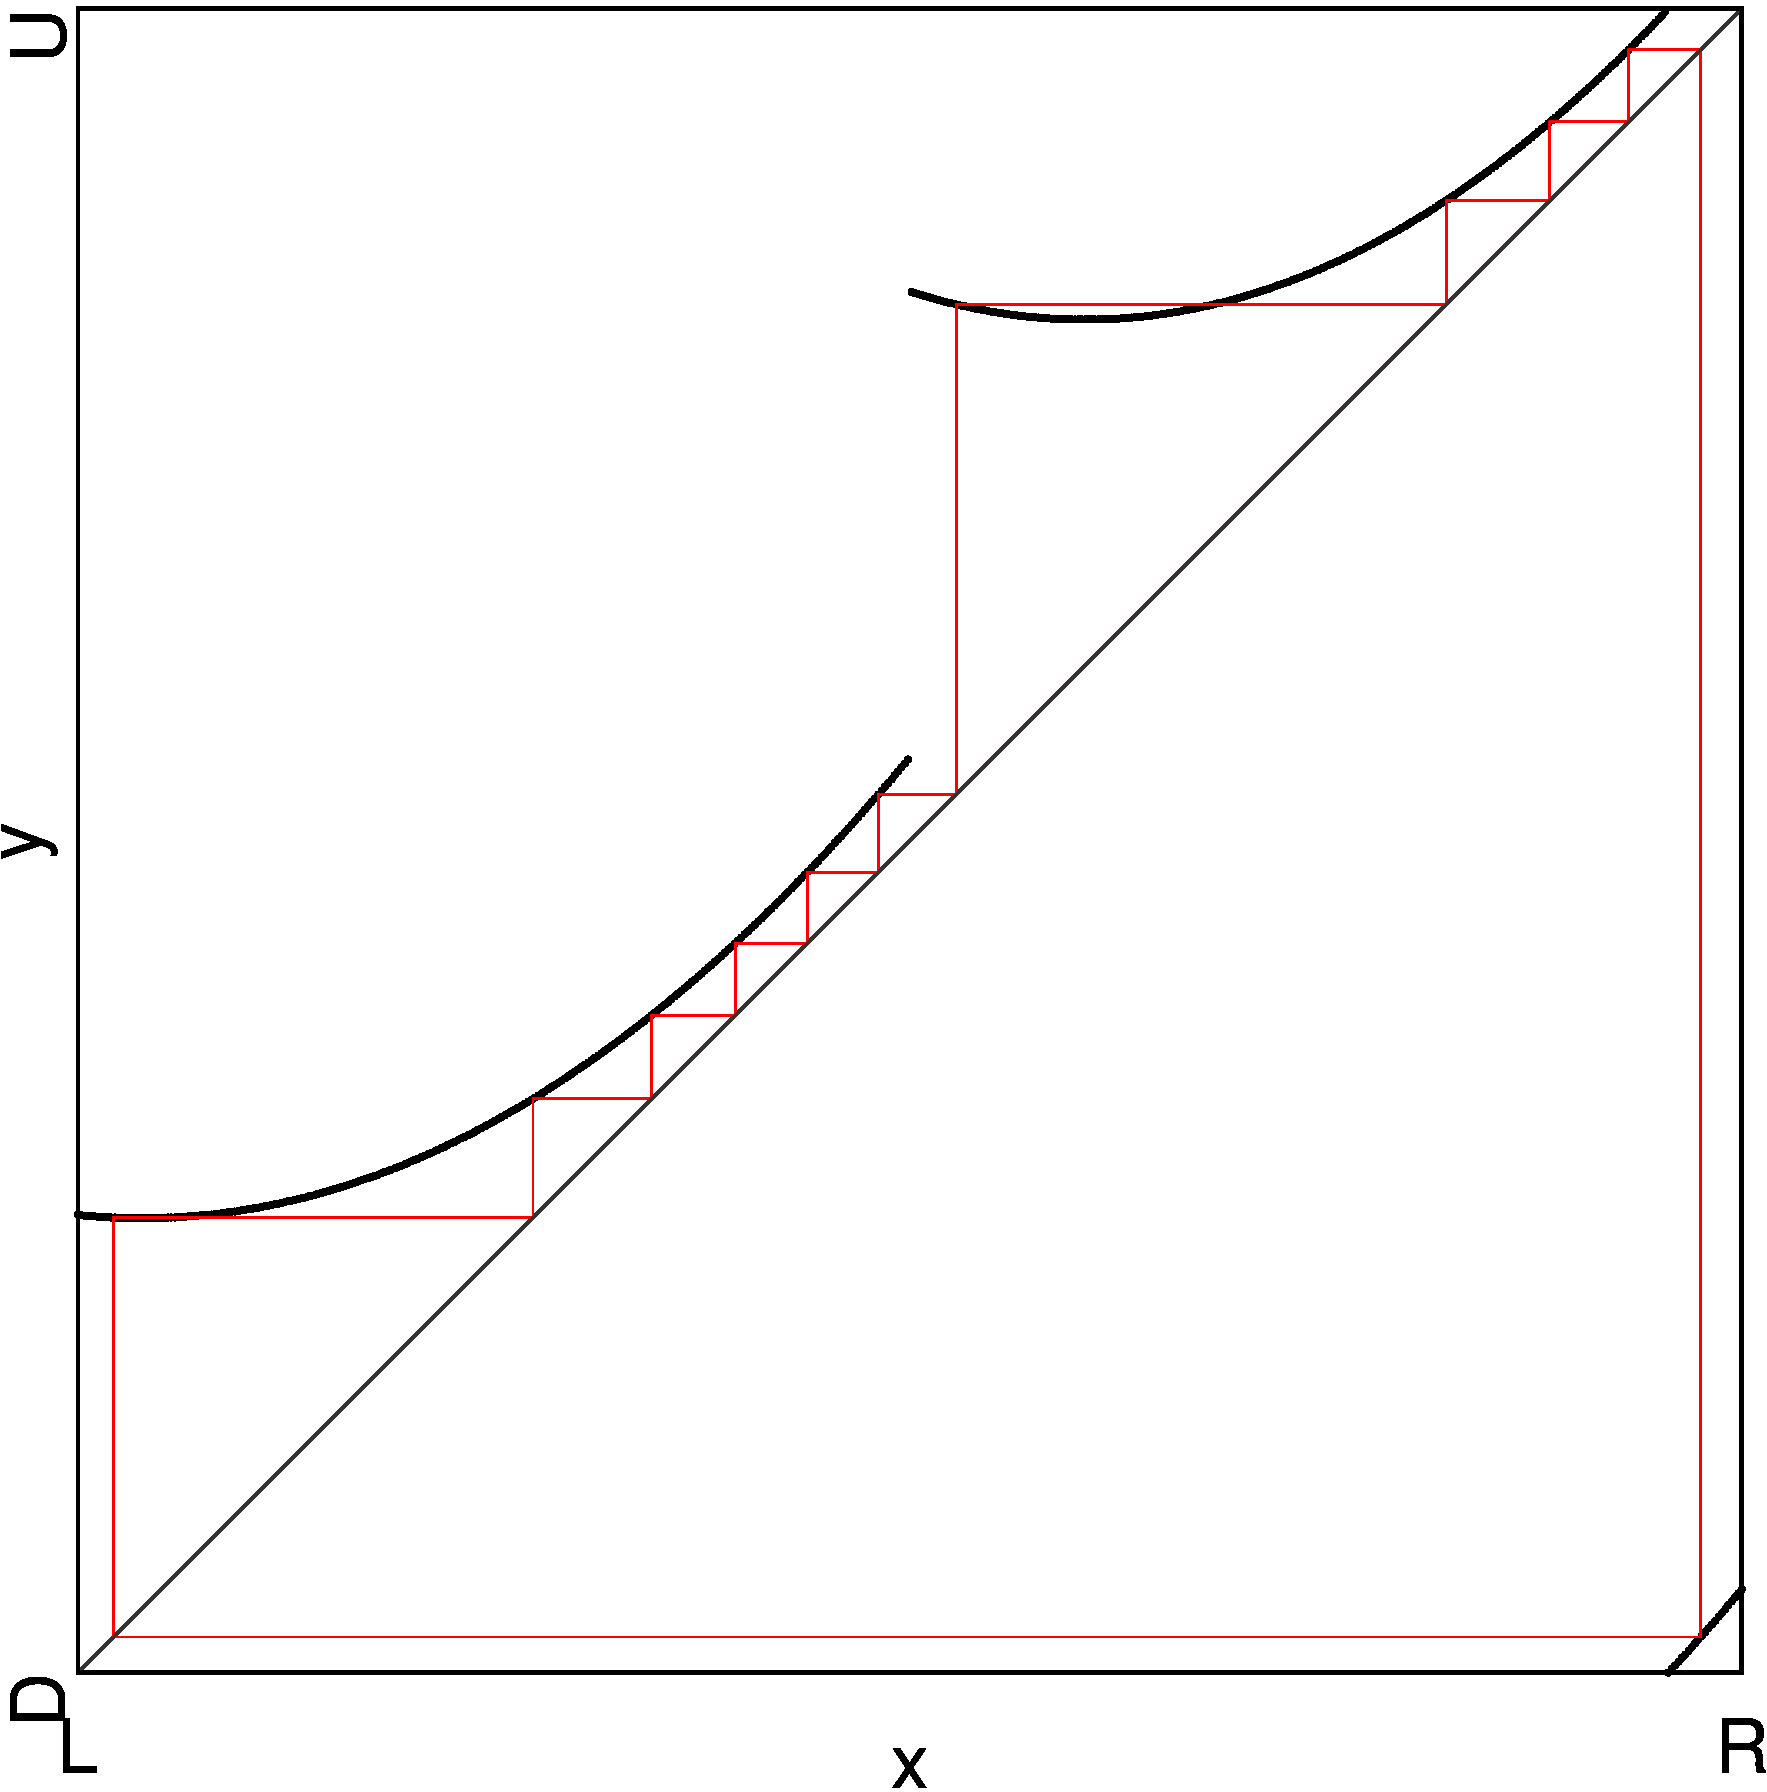
\includegraphics[width=.7 \textwidth]{63_MinimalRepr_Adding_Halved/Cob_Vis_s/Manual/result.png}
	\caption{Illustration of the infinite model concept.}
	\label{fig:minrep.infinite.model.concept}
\end{figure}

\subsubsection{Naive Algorithm}

Based on this concept of the infinite model, one can formulate a naive algorithm for translating symbolic sequences between the halved and full model.
We will start with the easier direction from the full to the halved model.
From this direction we can't learn much about the nature of the period-adding structure in the full model, the inverse will be more important for that.

To translate a symbolic sequence of the full model we start by writing it down.
For example $\A^4\B^3\C^4\D^3$.
Then we replace the symbols $\A$ and $\C$ by $\L$ and the symbols $\B$ and $\D$ by $\R$.
Now we have $\L^4\R^3\L^4\R^3$.
Finally, we have to check for redundancy in the resulting cycle.
In our example, the cycle $\L^4\R^3$ repeats twice in $\L^4\R^3\L^4\R^3$, so we just keep $\L^4\R^3$.
\todo{explain using the illustration}

The inverse is trickier.
We start by writing down the symbolic sequence in the halved model.
For example $\L^4\R^3\L4\R^3\L^3\R^3$.
Notice, this symbolic sequence has 3 rotations.
This means in the infinite model 3 red blocks are repeating.
To translate it to the full model, we have to fit the repeating blocks inside blue blocks.
But this does not work, since each blue block fits exactly 2 red blocks.
This means we have to write down the original sequence twice $\L^4\R^3\L4\R^3\L^3\R^3\L^4\R^3\L4\R^3\L^3\R^3$.
This is only necessary for sequences with an odd number of rotations, otherwise writing it down one is enough.

Then we pair up the rotations, this corresponds to drawing blue boxes around the red boxes in the infinite model.
In our example, we get the pairs $(\L^4\R^3\L^4\R^3)(\L^3\R^3\L^4\R^3)(\L^4\R^3\L^3\R^3)$.
The pairs then have to be translated using the function $t$ defined below.
The resulting symbolic sequence is $\A^4\B^3\C^4\D^3\A^3\B^3\C^4\D^3\A^4\B^3\C^3\D^3$.

\begin{definition}
	The function $t$ maps two rotations of a symbolic sequence in the halved model to a single rotation in the full model.
	It is defined in the following way.
	\begin{align}
		t: & \L^a\R^b\L^c\R^d \mapsto \A^a\B^b\C^c\D^d
	\end{align}
\end{definition}

\begin{definition}
	The function $s$ shifts a symbolic sequence in the halved model by a single rotation.
	Let $\tau_1\tau_2 \dots \tau_n$ be a sequence in the halved model, where each $\tau_i$ is one rotation.
	Then $s$ is defined in the following way.
	\begin{align}
		s: & \tau_1\tau_2 \dots \tau_n \mapsto \tau_2 \dots \tau_n\tau_1
	\end{align}
	In the full model, there is a similar function, $s'$, that shifts a symbolic sequence in the full model by a single rotation.
	Let $\tau'_1\tau'_2 \dots \tau'_n$ be a sequence in the full model, where each $\tau'_i$ is one rotation.
	The $s'$ is defined in the following way.
	\begin{align}
		s': & \tau'_1\tau'_2 \dots \tau'_n \mapsto \tau'_2 \dots \tau'_n\tau'_1
	\end{align}
\end{definition}

\begin{definition}
	The two symbolic sequences $\sigma$ and $\rho$ in the full model are shift-equivalent $\sigma \equiv \rho$,
	if they both have the same number of rotations $n$
	and there is a number $0 \leq i < n$, such that $\sigma = s'^i(\rho)$.
	Where $s'^i$ is the same as applying $s'$ $i$ times.
\end{definition}

We need to repeat the whole process for each shift $s^i$ of the original symbolic sequence for $0 < i < n$ where $n$ is the number of rotations of the original symbolic sequence.
And we only keep the results that are not shift-equivalent to any previous result.
In our example, we would repeat the process for $\L^4\R^3\L3\R^3\L^4\R^3$ and get the result $\A^4\B^3\C^3\D^3\A^4\B^3\C^4\D^3\A^3\B^3\C^4\D^3$.
This result is shift-equivalent to the first result by shifting it 2 times.
Last we need to repeat it for $\L^3\R^3\L4\R^3\L^4\R^3$ and get the result $\A^3\B^3\C^4\D^3\A^4\B^3\C^3\D^3\A^4\B^3\C^4\D^3$.
This result is shift-equivalent to the first result by rotating it once.

Therefore the cycle $\L^4R^3\L^4\R^3\L^3\R^3$ in the halved model manifests as a single cycle $\A^4\B^3\C^4\D^3\A^3\B^3\C^4\D^3\A^4\B^3\C^3\D^3$ in the full model.

\subsubsection{Insights}
\todo{better heading}

With this naive algorithm, we can start to investigate rules for the period-adding structure in the full model.

\begin{lemma}
	The translations of the two cycles $h_1$ and $h_2 = r^{2i}(h_1)$ in the halved model are equivalent $T(h_1) \equiv T(h_2)$ for all integers $i$.
\end{lemma}

\begin{proof}
	Let $h_1 = \tau_1\tau_2 \dots \tau_n$, therefore $h_2 = \tau_{2i+1} \dots \tau_n\tau_1 \dots \tau_{2i}$.
	The translations are $T(h_1) = t(\tau_1\tau_2)t(\tau_3\tau_4) \dots t(\tau_{n-1}\tau_n)$
	and $T(h_2) = t(\tau_{2i+1}\tau_{2i+2}) \dots t(\tau_{n-1}\tau_n)t(\tau_1\tau_2) \dots t(\tau_{2i-i}\tau_{2i})$.
	We can see that $T(h_2) = r'^i(T(h_1))$ and therefore $T(h_1) \equiv T(h_2)$.
\end{proof}

Therefore, we don't have to look at all rotations as a starting point for pairing, as described above.
It is enough to check both $T(h)$ and the once rotated case $T(r(h))$.
Therefore, each cycle in the halved model has at most 2 manifestations in the full model.

\subsubsection{Connections}
\todo{Better title}

\begin{theorem}
	A cycle in the halved model manifests either as a single cycle or two coexisting cycles in the full model.
\end{theorem}

\begin{theorem}
	\begin{enumerate}
		\item In the case of two coexisting cycles in the full model, the period of either cycle is half of the period of the cycle in the halved model: $|T(h)| = |T(r(h))| = \frac{1}{2} |h|$.
		\item In the case of one cycle in the full model, the period of this cycle is the same as the period of the cycle in the halved model: $|T(h)| = |T(r(h))| = |h|$.
	\end{enumerate}
\end{theorem}

\begin{theorem}
	\label{theorem:coex.even.odd}
	\begin{enumerate}
		\item The cycle $h$ manifests as two coexisting cycles in the full model, if and only if its number of rotations $n$ is even.
		\item The cycle $h$ manifests as one single cycle in the full model, if and only if its number of rotations $n$ is odd.
	\end{enumerate}
\end{theorem}

\begin{proof}
	\begin{enumerate}
		\item Let the number of rotations $n$ of $h$ be even
		      \begin{enumerate}[label=\alph*)]
			      \item Not rotated
			            \begin{align*}
				            T(h) & = t(\tau_1\tau_2) \dots t(\tau_{n-1}\tau_n) t(\tau_1\tau_2) \dots t(\tau_{n-1}\tau_n) \\
				                 & = (t(\tau_1\tau_2) \dots t(\tau_{n-1}\tau_n))^2                                       \\
				                 & \equiv t(\tau_1\tau_2) \dots t(\tau_{n-1}\tau_n) = a
			            \end{align*}
			      \item Rotated once
			            \begin{align*}
				            T(r(h)) & = t(\tau_2\tau_3) \dots t(\tau_{n}\tau_1) t(\tau_2\tau_3) \dots t(\tau_{n}\tau_1) \\
				                    & = (t(\tau_2\tau_3) \dots t(\tau_{n}\tau_1))^2                                     \\
				                    & \equiv t(\tau_2\tau_3) \dots t(\tau_{n}\tau_1) = b
			            \end{align*}
		      \end{enumerate}
		      We can see that $a \nequiv b$, unless $\tau_1 = \tau_2 = \tau_3 = \dots = \tau_n$.
		      For our adding structures, there must exist two integers $i, j$, for which $\tau_i \neq \tau_j$.
		      Also, we can see that the periods of the translated cycles are the same as the period of the original cycle.
		      The function $t$ preserves the period of the cycle, so $|\L^a\R^b\L^c\R^d| = a + b + c + d = |t(\L^a\R^b\L^c\R^d)| = |\A^a\B^b\C^c\D^d|$.
		      \begin{align*}
			      |a| & = |t(\tau_1\tau_2) \dots t(\tau_{n-1}\tau_n)|                                                       \\
			          & = \frac{1}{2} |(t(\tau_1\tau_2) \dots t(\tau_{n-1}\tau_n))^2|                                       \\
			          & = \frac{1}{2} |t(\tau_1\tau_2) \dots t(\tau_{n-1}\tau_n) t(\tau_1\tau_2) \dots t(\tau_{n-1}\tau_n)| \\
			          & = \frac{1}{2} |\tau_1\tau_2 \dots \tau_n\tau_1 \dots \tau_n|                                        \\
			          & = |\tau_1\tau_2 \dots \tau_n| = |h|
		      \end{align*}
		      Analogously for $|b| = |h|$.
		\item Let the number of rotations $n$ of $h$ be odd
		      \begin{enumerate}[label=\alph*)]
			      \item Not rotated
			            \begin{align*}
				            T(h) & = t(\tau_1\tau_2) \dots t(\tau_{n}\tau_1) t(\tau_2\tau_3) \dots t(\tau_{n-1}\tau_n) = a
			            \end{align*}
			      \item Rotated once
			            \begin{align*}
				            T(r(h)) & = t(\tau_2\tau_3) \dots t(\tau_{n-1}\tau_n) t(\tau_1\tau_2) \dots t(\tau_{n-1}\tau_n) = b
			            \end{align*}
		      \end{enumerate}
		      We can see that $a = r'^{\frac{n+1}{2}}(b)$ and therefore $a \equiv b$.
		      This means, that the cycle $h$ manifests as a single cycle in the full model.
		      Also, we can see that the period of the translated cycle is double the period of the original cycle.
		      \begin{align*}
			      |a| & = |t(\tau_1\tau_2) \dots t(\tau_n\tau_1) \dots t(\tau_{n-1}\tau_n)| \\
			          & = |\tau_1\tau_2 \dots \tau_n\tau_1 \dots \tau_{n-1}\tau_n|          \\
			          & = 2 |\tau_1\tau_2 \dots \tau_n| = 2 |h|
		      \end{align*}
		      Analogously for $|b| = 2 |h|$.
	\end{enumerate}
\end{proof}

Looking at the farey tree in \Cref{fig:tree.adding1.hor.full}, we can see some regularities in the distribution of coexisting (yellow) and single (white) cycles in the full model.
These can be explained with \Cref{theorem:coex.even.odd}.
%The third case in the theorem can't be seen in the farey tree, because we did not go deep enough into the tree but follows from the logic.

\begin{theorem}
	\begin{enumerate}
		\item The simultaneous child of a node with a single cycle and a node with two coexisting cycles has a single cycle.
		\item The simultaneous child of two nodes with a single cycle has two coexisting cycles.
		      %		\item The simultaneous child of two nodes with two coexisting cycles, has two coexisting cycles.
	\end{enumerate}
\end{theorem}

\begin{proof}
	\begin{enumerate}
		\item A node with a single cycle in the full model is the manifestation of a cycle with an odd number of rotations in the halved model.
		      A node with two coexisting cycles in the full model is the manifestation of a cycle with an even number of rotations in the halved model.
		      Their simultaneous child is the manifestation of the two cycles in the halved model glued together.
		      This glued-together cycle has an odd number of rotations and therefore manifests as a single cycle in the full model.
		\item Analogously, two cycles with an odd number of rotations glued together have an even number of rotations.
		      Therefore, this glued-together cycle manifests as two coexisting cycles in the full model.
		      %		\item Analogously, two cycles with an even number of rotations glued toghether have an even number of rotations.
		      %		      Therefore this glued toghether cycle manifests as two coexisting cycles in the full model.
	\end{enumerate}
\end{proof}

\todo{Improved algorithm?}
